\chapter{Implementaciones clásicas}

\begin{chapquote}{Emile Michel Cioran, \textit{Silogismos de la amargura}}
Sólo los espíritus agrietados poseen aberturas al más allá.
\end{chapquote}

En principio, se ha elaborado un prototipo en \textit{Haskell} del algoritmo \textit{DPLL}, usando la representación \textit{CNF} y otro para la conversión de fórmulas proposicionales a \textit{BDDs}. Ambos usando como base el mismo modelo de representación para la proposiciones lógicas usando tipos de datos algebraicos, pero realizando una un proceso de conversión diferente. Esto con el objetivo de tener una prueba conceptual de soluciones que existen actualmente para \sat.

\section{Proposiciones lógicas en \textit{Haskell}}
\label{sec:data}

Como primer paso se ha decidido representar a las proposiciones lógicas en \textit{Haskell} de forma arborescente, con un tipo de dato algebraico recursivo que puede verse en la figura \ref{code:prop}. En donde se han definido operadores, que son realmente constructores del tipo, y tienen una precedencia asignada que va en concordancia con la de los operadores lógicos de conjunción (\texttt{:\&:}), disyunción (\texttt{:|:}), implicación (\texttt{:>:}) y equivalencia (\texttt{:=:}). La negación posee un constructor usual y al igual que las sentencias de la proposición. A partir de esta definición se basan todos los algoritmos que se han implementado y resulta la forma más natural de hacerlo en \textit{Haskell}.

\begin{figure}
\begin{lstlisting}[language=Haskell]
    data Prop a
        = (Prop a) :&: (Prop a)
        | (Prop a) :|: (Prop a)
        | (Prop a) :>: (Prop a)
        | (Prop a) :=: (Prop a)
        | Neg (Prop a)
        | Stmnt a
\end{lstlisting}
\caption{Tipo de dato \textit{Haskell} para proposiciones lógicas.}
\label{code:prop}
\end{figure}

\section{\textit{CNF}}

Esta representación separa a una fórmula lógica en cláusulas operadas por la operación ($\land$), reduciendo el problema \sat a buscar la cláusula que no se cumpla dada cierta asignación de valores booleanos a las variables. Es evidente que se irían verificando las cláusulas hasta que alguna falle, en ese momento se sabría que esa combinación de valores para la proposición no es satisfactible.

El proceso de normalización comienza obteniendo la forma normal negativa (\textit{NNF}) de la proposición lógica para luego aplicar la propiedad distributiva del ($\lor$) sobre ($\land$) hasta que no se pueda aplicar más. Los algoritmos para obtener la \textit{NNF} y \textit{CNF} pueden verse en la figuras \ref{code:nnf} y \ref{code:cnf} respectivamente\cite{huth2004logic}, donde la función \texttt{DISTR} es quien aplica la propiedad distributiva; definida en la figura \ref{code:distr}. Previamente se necesita que la fórmula esté libre de implicaciones a través del siguiente teorema. \[ p \implies q \equiv \neg p \lor q \]

\begin{figure}
\begin{lstlisting}[language=C,mathescape=true,keywordstyle=\color{black}]
    function NNF($\phi$):
    /* $\phi$ está libre de implicaciones */
    /* NNF($\phi$) obtiene una NNF para $\phi$ */
    begin function
        case
            $\phi$ es una sentencia: return $\phi$
            $\phi$ es $\neg\neg\phi_1$: return NNF($\phi_1$)
            $\phi$ es $\phi_1 \land \phi_2$: return NNF($\phi_1$) $\land$ NNF($\phi_2$)
            $\phi$ es $\phi_1 \lor \phi_2$: return NNF($\phi_1$) $\lor$ NNF($\phi_2$)
            $\phi$ es $\neg(\phi_1 \land \phi_2)$: return NNF($\neg\phi_1$) $\lor$ NNF($\neg\phi_2$)
            $\phi$ es $\neg(\phi_1 \lor \phi_2)$: return NNF($\neg\phi_1$) $\land$ NNF($\neg\phi_2$)
        end case
    end function
\end{lstlisting}
\caption{Algoritmo para obetener la \textit{NNF}.}
\label{code:nnf}
\end{figure}

\begin{figure}
\begin{lstlisting}[language=C,mathescape=true,keywordstyle=\color{black}]
    function CNF($\phi$):
    /* $\phi$ está libre de implicaciones y en NNF */
    /* CNF($\phi$) obtiene una CNF equivalente para $\phi$ */
    begin function
        case
            $\phi$ es una sentencia: return $\phi$
            $\phi$ es $\phi_1 \land \phi_2$: return CNF($\phi_1$) $\land$ CNF($\phi_2$)
            $\phi$ es $\phi_1 \lor \phi_2$: return DISTR(CNF($\phi_1$), CNF($\phi_2$))
        end case
    end function
\end{lstlisting}
\caption{Algoritmo para obetener la \textit{CNF}.}
\label{code:cnf}
\end{figure}

\begin{figure}
\begin{lstlisting}[language=C,mathescape=true,keywordstyle=\color{black}]
    function DISTR($\eta_1$,$\eta_2$):
    /* $\eta_1$ y $\eta_2$ están en CNF */
    /* DISTR($\eta_1$,$\eta_2$) obtiene una CNF para $\eta_1 \lor \eta_2$ */
    begin function
        case
            $\eta_1$ es $\eta_{11} \land \eta_{12}$: return DISTR($\eta_{11}$,$\eta_{2}$) $\land$ DISTR($\eta_{12}$,$\eta_{2}$)
            $\eta_2$ es $\eta_{21} \land \eta_{22}$: return DISTR($\eta_1$,$\eta_{21}$) $\land$ DISTR($\eta_1$,$\eta_{22}$)
            en otro caso: return $\eta_1 \lor \eta_2$
        end case
    end function
\end{lstlisting}
\caption{Algoritmo para obetener la \textit{CNF} entre dos proposiones.}
\label{code:distr}
\end{figure}

\subsection{\textit{DPLL}}

El algortimo \textit{Davis–Putnam–Logemann–Loveland} (\textit{DPLL})\cite{Davis} está basado en el comportamiento de \textit{CNF}, este realiza una busqueda usando \textit{backtracking}, donde en cada paso hay se toma una desición y se examinan las cláusulas que conforman a la proposición lógica. La implementación en \textit{Haskell} reside en una función que se llama recursivamente tomando una desición de asignación en cada paso para alguna variable. Evalua las cláusulas para descartar aquellas que ya se tiene certeza de su satisfactibilidad y en caso de que alguna falle, la función retorna directamente \texttt{False}. Aprovechando la evaluación perezosa para dividir desiciones de asignación binaria en una simple disyunción.

En la figura \ref{code:dpll} se muestra un código representativo de lo que sucede en la implmentación del algoritmo \textit{DPLL}. Está definida para recibir tres argumentos, un \textit{hash} de desiciones, una lista de sentencias sin ningún valor (\texttt{True} o \texttt{False}) asignado, una lista de cláusulas (provenientes de una conversión a \textit{CNF}) y retornando un booleano. Existen tres posibles casos, los cuales se describen a continuación.

\begin{itemize}
    \item \textbf{Caso 0}: Si no falta una cláusula por comprobar su satisfactibilidad, entonces se puede decir que el algoritmo ha logrado encontrar una combinación de valores para las variables, que logran satisfacer las cláusulas.
    \item \textbf{Caso 1}: Si faltan cláusulas por satisfacer, y no hay más variables a las que se les pueda asignar algún valor, entonces se debe comprobar si con las desiciones tomadas hasta el momento se logran satisfacer todas. En el caso que no sea posible, se retorna \texttt{False}.
    \item \textbf{Caso 2}: Si faltan cláusulas por satisfacer, y aun quedan variables sin desición para su valor, entonces se evaluan las desiciones actuales en todas las cláusulas. Esto puede resultar en dos opciones, se consigue una nueva lista de cláusulas o alguna falla (representado por \texttt{Nothing}). La primera opción es la que genera una bifurcación para el valor que pueda tomar una variable sin asignar, en nuestro caso es la primera de la lista, y continua la ejecución a través de dos llamadas recursivas para las dos posibles desiciones; usando la nueva lista de cláusulas. La segunda opción sería simplemente retornar \texttt{False}, ya que alguna ha fallado.
\end{itemize}

\begin{figure}
\begin{lstlisting}[language=Haskell]
    dpll :: Map (a,Bool) -> [a] -> [Prop a] -> Bool
    dpll   _      _ [] = True -- Caso 0
    dpll hsh     [] ps = ...  -- Caso 1
    dpll hsh (s:ss) ps =      -- Caso 2
        case evalDecisions hsh ps of
            Just nps -> dpll  ((s,True):hsh) ss nps ||
                        dpll ((s,False):hsh) ss nps
            Nothing -> False
\end{lstlisting}
\caption{Algoritmo DPLL en \textit{Haskell}.}
\label{code:dpll}
\end{figure}

\section{\textit{BDDs}}
\label{sec:bdds}

Los diagramas binarios de desición (\textit{BDDs}) son una representación que se asemeja a un grafo dirigido acíclico, y resultan útiles porque tienen un comportamiento incremental. Se puede operar entre ellos y producir un nuevo \textit{BDD}, el cual unirá las proposiciones que representen los \textit{BDDs} originales, manteniendo orden y unicidad. Característica compartido con el polinomio de \textit{Zhegalkin}, lo cual veremos en el siguiente capítulo. Esta comportamiento es consecuencia de estructuras \textbf{normalizadas} y únicas para un determinado conjunto de condiciones. Esto tiene una ventaja cuando se va construyendo a partir de restricciones que van incorporándose a medida que el modelo del problema lo necesite. Sin necesidad de contruir nuevamente la estructura, si se incluye otra restricción al problema que se desea modelar.

\begin{figure}
    \begin{minipage}{0.45\textwidth}
    \centering
    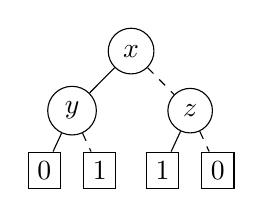
\begin{tikzpicture}
    [edge from parent/.style={draw=none}]
    \node[circle,draw](x){$x$}[level distance=5ex]
    child{node[circle,draw](y){$y$}[sibling distance=2em]
      child{node[draw](y0){$0$}}
      child{node[draw](y1){$1$}}
    }
    child{node[circle,draw](z){$z$} [sibling distance=2em]
      child{node[draw](z1){$1$}}
      child{node[draw](z0){$0$}}
    };
    \draw[dashed] (x) -- (z);
    \draw[dashed] (y) -- (y1);
    \draw[dashed] (z) -- (z0);
    \draw[solid] (x) -- (y);
    \draw[solid] (y) -- (y0);
    \draw[solid] (z) -- (z1);
    \end{tikzpicture}
\caption{Ejemplo 1 de \textit{BDD}.}
\label{fig:bdd_ex_1}
\end{minipage}\hfill
\begin{minipage}{0.45\textwidth}
    \centering
    \begin{tikzpicture}
    [edge from parent/.style={draw=none}]
    \node[circle,draw](w){$w$}[level distance=5ex]
        child{node[circle,draw](z){$z$} [sibling distance=2em]
            child{node[draw](z1){$1$}}
            child{node[draw](z0){$0$}}}
        child{node[draw](w0){$0$}};
    \draw[dashed] (w) -- (w0);
    \draw[dashed] (z) -- (z0);
    \draw[solid] (x) -- (y);
    \draw[solid] (z) -- (z1);
    \end{tikzpicture}
\caption{Ejemplo 2 de \textit{BDD}.}
\label{fig:bdd_ex_2}
\end{minipage}
\end{figure}


En la figura \ref{fig:bdd_ex_1} se puede ver un ejemplo de un \textit{BDD} construido a partir de la proposición $(x \land \neg y) \lor (\neg x \land z)$, es importante resaltar que se respeta el orden $x < y < z$. Si se tiene otro \textit{BDD}, como el que muestra la figura \ref{fig:bdd_ex_2}, que representa a la proposición $w \land z$ y se operan ambos por el operador de conjunción, el \textit{BDD} resultante sería el que se muestra en la figura \ref{fig:bdd_r}.

\begin{figure}
    \centering
    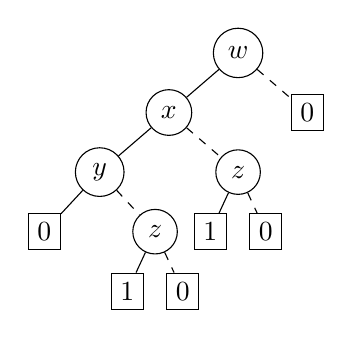
\begin{tikzpicture}
    [edge from parent/.style={draw=none}]
    \node[circle,draw](w){$w$}[level distance=5ex][sibling distance=5em]
        child{node[circle,draw](x){$x$} [level distance=5ex][sibling distance=5em]
            child{node[circle,draw](y){$y$} [level distance=5ex][sibling distance=4em]
                child{node[draw](y0){$0$}}
                child{node[circle,draw](z){$z$} [sibling distance=2em]
                    child{node[draw](z1){$1$}}
                    child{node[draw](z0){$0$}};
                };
            }
            child{node[circle,draw](zz){$z$} [sibling distance=2em]
                child{node[draw](zz1){$1$}}
                child{node[draw](zz0){$0$}};
            }
        }
        child{node[draw](w0){$0$}};
    \draw[dashed] (w) -- (w0);
    \draw[dashed] (x) -- (zz);
    \draw[dashed] (z) -- (z0);
    \draw[dashed] (zz) -- (zz0);
    \draw[dashed] (y) -- (z);
    \draw[solid] (w) -- (x);
    \draw[solid] (x) -- (y);
    \draw[solid] (y) -- (y0);
    \draw[solid] (z) -- (z1);
    \draw[solid] (zz) -- (zz1);
    \end{tikzpicture}
\caption{\textit{BDD} resultante de la conjunción.}
\label{fig:bdd_r}
\end{figure}

Para construir un \textit{BDD} a partir de una proposición booleana, usando el mismo tipo de dato definido en la figura \ref{code:prop}, se ha definido un tipo de dato que se puede ver en la figura \ref{code:bdds}, además se cuenta con una serie de operadores booleanos para operar con \textit{BDDs} y así poder tener una construcción incremental a partir de una fórmula lógica.

\begin{figure}
\begin{lstlisting}[language=Haskell]
data BDD a where
    Decision :: Ord a => Prop a -> BDD a -> BDD a -> BDD a
    Yes :: Ord a => BDD a
    No :: Ord a => BDD a
deriving instance Eq (BDD a)
\end{lstlisting}
\caption{Tipo de dato para \textit{BDDs} en \textit{Haskell}.}
\label{code:bdds}
\end{figure}

El tipo de dato para los \textit{BDDs} es arborescente y posee tres constructores de tipo, dos para los casos base y uno que es recursivo, donde también se almacena la proposición que representa. Al final, esa proposición, será una sentencia a cualquier nivel del árbol. Los operadores para este tipo de dato son un equivalente para la negación ($\neg$), conjunción ($\land$), disyunción ($\lor$), implicación ($\implies$) y equivalencia ($\iff$). Estos se pueden muestran en las figuras \ref{code:bdd_neg}, \ref{code:bdd_and}, \ref{code:bdd_or}, \ref{code:bdd_implies} y \ref{code:bdd_eq} respectivamente.

La función \texttt{apply} que se muestra en la figura \ref{code:bdd_apply} efectúa una comparación de las proposiciones almacenadas por cada \textit{BDD}, le da prioridad a la menor y reducirá en el caso de que la operación encuentre la oportunidad de eliminar un árbol. Esto es posible ya que si dos subárboles son iguales para una misma sentencia, las desiciones serán iguales independientemente de que valor tome esa sentencia y por eso es equivalente a un solo subárbol.

Los \textit{BDDs} pueden tener muchas utilidades, ya que indican facilmente si una proposición lógica se satisface o no, asi como los valores necesarios para que se satisfga. Pero en lo que se refiere a \sat, resulta costoso mantener una estructura arborescente ordenada y dado que el objetivo es paralelizar procesos, no se consideró oportuno como una opción para implementar con OpenCL.

\begin{figure}
\begin{lstlisting}[language=Haskell]
neg :: BDD a -> BDD a
neg No = Yes
neg Yes = No
neg (Decision v y n) = Decision v (neg y) (neg n)
\end{lstlisting}
\caption{Operación de negación para \textit{BDDs}.}
\label{code:bdd_neg}
\end{figure}

\begin{figure}
\begin{lstlisting}[language=Haskell]
and :: BDD a -> BDD a -> BDD a
and No _ = No
and _ No = No
and Yes d = d
and d Yes = d
and bdd1 bdd2 = apply and bdd1 bdd2
\end{lstlisting}
\caption{Operación de conjunción para \textit{BDDs}.}
\label{code:bdd_and}
\end{figure}

\begin{figure}
\begin{lstlisting}[language=Haskell]
or :: BDD a -> BDD a -> BDD a
or Yes _ = Yes
or _ Yes = Yes
or No d = d
or d No = d
or bdd1 bdd2 = apply or bdd1 bdd2
\end{lstlisting}
\caption{Operación de disyunción para \textit{BDDs}.}
\label{code:bdd_or}
\end{figure}

\begin{figure}
\begin{lstlisting}[language=Haskell]
implies :: BDD a -> BDD a -> BDD a
implies No  _ = Yes
implies Yes d = d
implies bdd1 bdd2 = or (neg bdd1) bdd2
\end{lstlisting}
\caption{Operación de implicación para \textit{BDDs}.}
\label{code:bdd_implies}
\end{figure}

\begin{figure}
\begin{lstlisting}[language=Haskell]
eq :: BDD a -> BDD a -> BDD a
eq No d = neg d
eq d No = neg d
eq Yes d = d
eq d Yes = d
eq bdd1 bdd2 = apply eq bdd1 bdd2
\end{lstlisting}
\caption{Operación de equivalencia para \textit{BDDs}.}
\label{code:bdd_eq}
\end{figure}


\begin{figure}
\begin{lstlisting}[language=Haskell]
apply :: (BDD a -> BDD a -> BDD a) -> BDD a -> BDD a -> BDD a
apply op bdd1@(Decision x1 y1 n1) bdd2@(Decision x2 y2 n2)
    | x1 < x2 =
        let
            ldd = op y1 bdd2
            rdd = op n1 bdd2
        in
            if ldd == rdd then ldd else Decision x1 ldd rdd
    | x1 > x2 =
        let
            ldd = op y2 bdd1
            rdd = op n2 bdd1
        in
            if ldd == rdd then ldd else Decision x2 ldd rdd
    | otherwise =
        let
            ldd = (op y1 y2)
            rdd = (op n1 n2)
        in
            if ldd == rdd then ldd else Decision x1 ldd rdd
\end{lstlisting}
\caption{Función \texttt{apply} para \textit{BDDs}.}
\label{code:bdd_apply}
\end{figure}

